\documentclass{article}

\PassOptionsToPackage{numbers}{natbib}
\usepackage[preprint]{neurips_2026}

\usepackage[utf8]{inputenc}
\usepackage[T1]{fontenc}
\usepackage{hyperref}
\usepackage{url}
\usepackage{booktabs}
\usepackage{amsfonts}
\usepackage{amsmath}
\usepackage{nicefrac}
\usepackage{microtype}
\usepackage{xcolor}
\usepackage{graphicx}
\usepackage{enumitem}
\usepackage{float}

\title{Can Adding Asymmetric Relation Dynamics Make Knowledge Transfer More Efficient in Language Agents?}

\author{
  Rishi More (\texttt{rmore2}) \\
  Department of Computer Science\\
  Johns Hopkins University\\
  \texttt{rmore2@jhu.edu}
}

\begin{document}

\maketitle

\begin{abstract}
Human intelligence develops within social relationships, yet language agent training ignores the relational structure between teacher and learner. This project investigates whether an asymmetric caregiver--child relationship improves knowledge transfer in language agents. I implement a cognitively-inspired memory architecture (instinct buffer, working memory, long-term episodic store, LoRA-based habits) and a salience-gated consolidation mechanism grounded in natural pedagogy theory, then compare four conditions---Solo, Symmetric Peer, Role-Labeled, and Relational---across 160 training episodes and 40 held-out transfer tasks. Results show that caregiver-assisted conditions achieve near-perfect training success (100\% vs.\ 82\%) with 25\% fewer dialogue turns, but this advantage does not fully transfer to independent evaluation---mirroring the ``scaffolding dependency'' phenomenon in developmental psychology. Qualitative analysis reveals that LLM agents exhibit fundamentally different failure modes from human children, including inability to learn from repeated corrections and absence of genuine causal reasoning, suggesting that role-playing social cognition in LLMs is shallow compared to human social learning.
\end{abstract}

\section{Introduction}

Human learning is fundamentally relational. From infancy, caregivers curate the information stream a child receives, selectively highlighting what is novel, correcting misconceptions, and adjusting explanations to the child's current understanding~\citep{csibra2009natural, gweon2021inferential}. Natural pedagogy theory~\citep{csibra2009natural} posits that humans are uniquely adapted to both teach and be taught: caregivers \emph{ostensively} signal when information is generic and worth storing, while learners are biased to encode information delivered in pedagogical frames. This cooperative inference process~\citep{gweon2021inferential} produces faster learning than passive observation~\citep{ho2019cooperative}.

Yet the relational structure between teacher and learner---the fact that a persistent \emph{relationship} shapes what gets taught and remembered---is absent from how language agents are trained today. This project asks: \textbf{does learning in an asymmetric relational dynamic (such as a caregiver--child structure) enable a language agent to acquire richer and more generalizable knowledge than learning alone or from a symmetric peer?}

This question connects directly to several topics from the course. \textbf{Theory of Mind}: the caregiver must model the child's knowledge state to select appropriate hints~\citep{baker2017rational}. \textbf{Cooperative communication}: teaching requires Gricean informativeness---saying what the learner needs, not everything the teacher knows. \textbf{Social learning}: the child learns from observing and interacting with the caregiver, not just from task rewards. \textbf{Mental state attribution}: the salience signal encodes whether the caregiver's pedagogical intent was present. The framework also relates to \textbf{rational action understanding}: a child who has internalized a model of the caregiver should be able to predict teaching actions as goal-directed behavior aimed at filling knowledge gaps~\citep{baker2017rational}.

\section{Problem formulation}

\subsection{Definitions and assumptions}

We define \textbf{asymmetric relational dynamics} as a persistent teacher--learner interaction where: (a)~the teacher has strictly more knowledge than the learner (information asymmetry), (b)~both agents maintain memory of past interactions (persistent relationship), and (c)~the teacher adapts its pedagogy to the learner's current competence (adaptive scaffolding). We assume that this structure, when combined with a salience-gated memory consolidation mechanism, will produce more robust and generalizable learning than conditions lacking one or more of these properties.

\textbf{Hypotheses.} \textbf{H1}: The relational child achieves higher transfer accuracy on held-out tasks than solo or peer conditions. \textbf{H2}: Caregiver-assisted conditions form habits (LoRA updates) faster. \textbf{H3}: The relational child internalizes a rudimentary model of the caregiver's pedagogical strategy (ToM proxy).

\subsection{Task environment}

I constructed 197 procedural household tasks spanning 10 categories (cleaning, cooking, home repair, etc.) and 8 difficulty levels (1--8 action steps). Tasks were generated via a multi-stage pipeline using Qwen3-235B-A22B-Instruct: (1)~object ontology generation, (2)~BM25-diversity-filtered skeleton generation, (3)~full task expansion with causally-ordered action sequences and graduated caregiver hints, and (4)~self-verification with catch-and-retry. The final dataset is split 157/40 for training/evaluation.

\subsection{Agent memory architecture}

Each agent maintains four memory components, inspired by Tulving's taxonomy of memory systems~\citep{tulving1985memory}:

\begin{itemize}[leftmargin=*,itemsep=1pt]
    \item \textbf{M1. Instinct buffer} ($\mathcal{I}$): A fixed system prompt encoding role-specific behavioral priors. Never updated during training.
    \item \textbf{M2. Working memory} ($\mathcal{W}_t$): A sliding window of the last $k{=}8$ dialogue turns.
    \item \textbf{M3. Long-term memory} ($\mathcal{L}$): An episodic store compressed via 235B-model summarization. Retrieval uses BM25 keyword matching. New entries gated by salience $> \tau = 0.3$.
    \item \textbf{M4. Habit store} ($\mathcal{H}$): LoRA adapter weights (rank 16, lr$\,{=}\,2{\times}10^{-5}$) updated via salience-weighted SFT on successful trajectories, with batch accumulation (min 4 examples).
\end{itemize}

\subsection{Salience signal}

The consolidation gate uses a composite salience score:
\[
s = \alpha \cdot \text{novelty}(e) + \beta \cdot \text{pred\_error}(e) + \gamma \cdot \text{teaching}(e)
\]

\textbf{Novelty} ($\alpha{=}0.3$): category frequency decay $\frac{1}{1+\text{count}}$ combined with BM25 task-level distance to stored LTM entries. \textbf{Prediction error} ($\beta{=}0.4$): Rescorla-Wagner surprise $|r - \bar{r}_\text{cat}|$ plus zone-of-proximal-development (ZPD) matching via Gaussian centered at $r{=}0.5$~\citep{wood1976role}. \textbf{Teaching signal} ($\gamma{=}0.3$): productive struggle (correction$\to$improvement patterns in partial credits) plus effort ratio. In non-caregiver conditions, $\gamma = 0$.

\subsection{Interaction protocol and scaffolding}

The caregiver (Qwen3-235B, frozen) has full task access and provides adaptive scaffolding based on the child's rolling competence per category: \emph{full support} (competence $<0.3$: step-by-step hints), \emph{guided discovery} ($0.3$--$0.7$: Socratic questions and partial hints), or \emph{minimal support} ($>0.7$: brief confirmation). The child (Qwen3-8B + LoRA) has no solution access. A semantic action judge (235B) evaluates each child action against ground-truth steps, providing partial credit scores and natural-language feedback.

\subsection{Experimental conditions}

\begin{table}[h]
  \caption{Four conditions isolating role asymmetry and relational salience. Each condition run with 3 random seeds across 160 episodes.}
  \label{tab:conditions}
  \centering
  \begin{tabular}{lll}
    \toprule
    \textbf{Condition} & \textbf{Agent structure} & \textbf{Teaching signal $\gamma$} \\
    \midrule
    Solo & Single 8B child, no partner & 0 \\
    Symmetric Peer & Two 8B agents, no roles & 0 \\
    Role-Labeled & 235B caregiver + 8B child & 0 \\
    Relational & 235B caregiver + 8B child & 0.3 \\
    \bottomrule
  \end{tabular}
\end{table}

\section{Related work}

\paragraph{Natural pedagogy and cooperative inference.} \citet{csibra2009natural} argue that human pedagogy involves ostensive signals that mark information as generic and worth encoding. \citet{gweon2021inferential} formalizes this as cooperative inference: the teacher selects demonstrations based on a model of the learner's knowledge, and the learner uses the teacher's selections as evidence. Our framework operationalizes these ideas via the caregiver's adaptive scaffolding (which requires implicit ToM) and the teaching signal in salience (which weights caregiver-guided episodes more heavily).

\paragraph{Theory of Mind in agents.} \citet{baker2017rational} formalize rational action understanding as Bayesian inverse planning over beliefs, desires, and percepts. Our H3 hypothesis tests whether the child agent develops a rudimentary ToM. \citet{lake2024building} argue that building machines that learn and think \emph{with} people requires social cognitive foundations that current models lack---our results support this view.

\paragraph{Scaffolding in education.} \citet{wood1976role} introduced scaffolding as a metaphor for how tutors adjust support. \citet{puntambekar2005tools} documented scaffolding dependency in educational technology, where learners who receive consistent support fail to develop independent strategies---precisely the phenomenon our H1 results reveal.

\paragraph{Memory and social cognition.} Generative Agents~\citep{park2023generative} use hierarchical memory with reflection but do not examine how social relationships shape memory formation. Our work adds salience-gated consolidation inspired by the finding that socially significant events occupy privileged positions in human episodic memory~\citep{dolcos2004interaction}. Character-LLM~\citep{shao2023character} shows that stable roles shift LLM response distributions, which our results confirm and extend.

\paragraph{LoRA as habit formation.} Parameter-efficient fine-tuning~\citep{hu2022lora} encodes behavioral adaptations that persist across contexts. We extend this to salience-weighted SFT where gradient magnitude is modulated by social context---novel relative to standard LoRA applications.

\section{Results}

\subsection{H1: Transfer accuracy --- not supported}

Transfer accuracy on 40 held-out tasks (Figure~\ref{fig:h1}) shows surprisingly small differences: Solo ($0.686 \pm 0.046$), Peer ($0.686 \pm 0.078$), Role-Labeled ($0.708 \pm 0.033$), and Relational ($0.682 \pm 0.087$). Despite dramatically different training success rates (Section~\ref{sec:h2}), child agents converge to similar held-out performance when tested independently without caregiver assistance.

\begin{figure}[h]
    \centering
    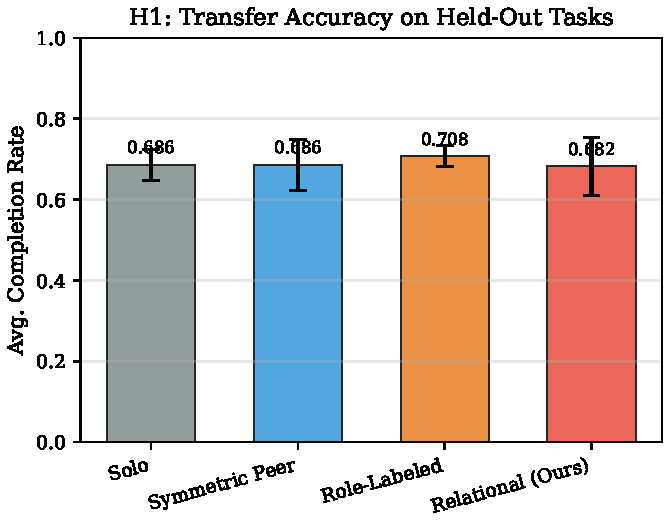
\includegraphics[width=0.85\linewidth]{figures/h1_transfer.pdf}
    \caption{Transfer accuracy on held-out tasks. All conditions achieve $\sim$0.68--0.71, with differences within noise. Error bars: std over 3 seeds.}
    \label{fig:h1}
\end{figure}

\subsection{H2: Habit acceleration --- strongly supported}
\label{sec:h2}

Caregiver-assisted conditions achieve near-perfect training success: 100\% (Role-Labeled) and 99.8\% (Relational) vs.\ 81.5\% (Solo) and 84.4\% (Peer). Caregiver conditions require 25\% fewer turns (6.1 vs.\ 8.4) and trigger all 160 LoRA updates vs.\ $\sim$130 for Solo/Peer (Figure~\ref{fig:h2}).

\begin{figure}[h]
    \centering
    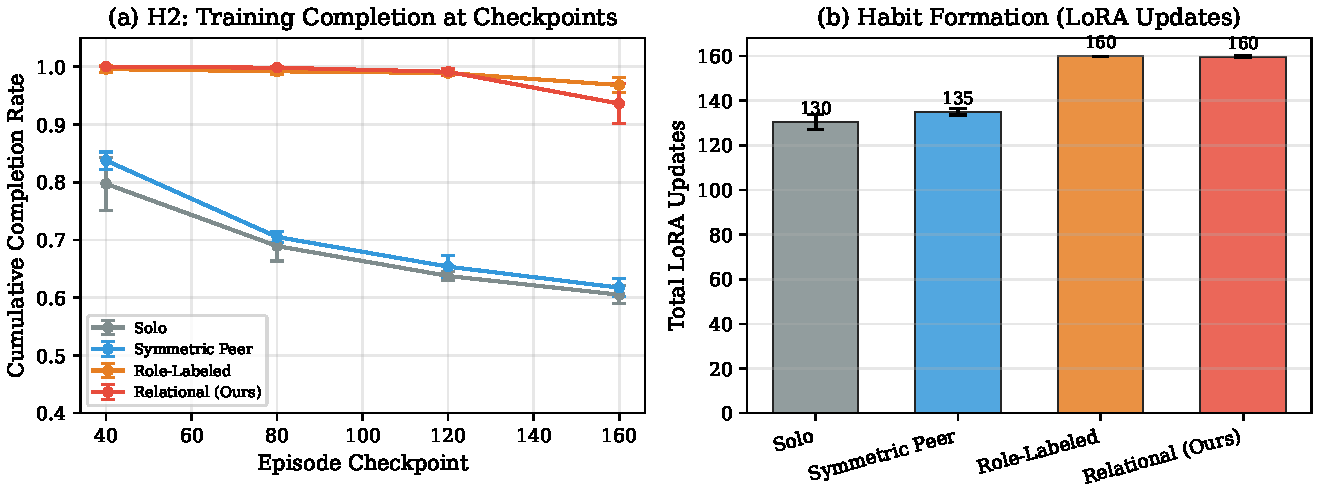
\includegraphics[width=\linewidth]{figures/training_success.pdf}
    \caption{(a) Cumulative training success. (b) LoRA updates. Caregiver conditions maintain $>$95\% success and trigger all 160 updates.}
    \label{fig:h2}
\end{figure}

\subsection{H3: Theory of Mind proxy --- not supported}

BM25 similarity between the child's predicted and actual caregiver utterances was $0.066 \pm 0.003$---near zero. We argue this is primarily a measurement limitation (see Section~\ref{sec:limitations}).

\begin{table}[h]
  \caption{Summary statistics across conditions (mean $\pm$ std over 3 seeds).}
  \label{tab:summary}
  \centering
  \small
  \begin{tabular}{lcccc}
    \toprule
    \textbf{Metric} & \textbf{Solo} & \textbf{Peer} & \textbf{Role-Labeled} & \textbf{Relational} \\
    \midrule
    H1 Transfer Accuracy & .686\tiny{$\pm$.046} & .686\tiny{$\pm$.078} & \textbf{.708}\tiny{$\pm$.033} & .682\tiny{$\pm$.087} \\
    Training Success Rate & 81.5\% & 84.4\% & \textbf{100\%} & 99.8\% \\
    Avg. Turns to Complete & 8.36 & 8.52 & \textbf{6.10} & 6.42 \\
    Total LoRA Updates & 130 & 135 & \textbf{160} & 160 \\
    H3 ToM (BM25 sim.) & --- & --- & --- & .066\tiny{$\pm$.003} \\
    \bottomrule
  \end{tabular}
\end{table}

\section{Qualitative analysis: successes and failures}

\subsection{Success: Relational scaffolding in action}

\textbf{Example 1: Laundry task (Relational, episode 46, difficulty 3).} The child was asked to ``sort a mixed load of whites and colors, wash the whites separately, and transfer them to the dryer.'' The child retrieved relevant past experiences from LTM---including a prior laundry episode where the caregiver demonstrated how to open the washing machine---and independently planned the full sequence: sort whites into the laundry basket, open the washing machine by pulling the handle, add detergent from the cabinet, wash, then transfer to dryer. The caregiver recognized the child's competence and provided minimal-support feedback: \emph{``I'm so proud of how carefully you planned the laundry---opening the machine, adding detergent, and remembering to check the dryer.''}

This episode demonstrates the ideal training trajectory: BM25-retrieved past experiences provide useful grounding, and the caregiver's support has appropriately faded from full guidance to encouragement.

\textbf{Example 2: Gardening task (Relational, episode 20, difficulty 2).} When fertilizing a potted lemon tree, the caregiver employed Socratic questioning: \emph{``When we mix something strong like concentrated liquid fertilizer, do we usually add it to water, or add water to it? What might happen in each case?''} The child reasoned: \emph{``If I add the concentrated fertilizer directly, it might be too strong and burn the roots. So I should pour a small amount into the watering can, then fill with water.''} This exemplifies cooperative communication where the teacher activates the learner's reasoning rather than transmitting the answer directly.

\subsection{Failure: Solo agent perseveration}

\textbf{Example 3: Home repair task (Solo, episode 3, difficulty 1).} The child was asked to tighten a loose screw on a cabinet door hinge---a 1-step task. Despite having relevant LTM from a prior bookshelf assembly episode (where the caregiver had explained that ``screws go in with the screwdriver, not the hammer''), the solo child spent all 4 turns generating lengthy \texttt{<think>} blocks reasoning about tool selection, screwdriver types, and screw rotation direction, but \emph{never produced a concrete executable action}. The judge marked each turn ``incorrect.'' Critically, the child repeated increasingly verbose versions of the \emph{same} reasoning across all 4 turns, unable to recognize that its approach was failing and pivot to a different strategy.

\subsection{Failure: Peer condition repetitive loops}

\textbf{Example 4: Gardening task (Peer, episode 20, difficulty 2).} Two 8B agents attempted to fertilize a lemon tree. Both independently arrived at the correct high-level plan (retrieve fertilizer from shed, dilute with water, apply to soil), but their outputs were formatted as multi-step bullet-point explanations rather than single executable actions. The judge evaluated each turn against one ground-truth step and marked them all incorrect. Both peers repeated the same full plan across all turns with minor rephrasing, never breaking their response into atomic actions. Without a more capable agent to model the correct interaction format, neither peer could adapt.

\section{Discussion}

\subsection{The scaffolding dependency effect}

The central finding is a striking dissociation: 100\% training success but no transfer advantage. This directly mirrors the \textbf{scaffolding dependency} phenomenon documented in developmental psychology~\citep{wood1976role}: when scaffolding is not systematically faded, learners become dependent on external support~\citep{puntambekar2005tools}. The LoRA weights encode behaviors optimized for the \emph{assisted} context; removing the caregiver at evaluation eliminates the real-time corrective feedback the child relied on.

Our adaptive scaffolding reduces hint specificity as competence grows but never fully withdraws---even at ``minimal support,'' the caregiver still responds each turn. A critical missing ingredient is \textbf{scaffolding fading}: progressively forcing the child to act independently during later training episodes, so the LoRA weights encode self-sufficient strategies.

\subsection{How these agents differ from human children}
\label{sec:agents_vs_humans}

The transcripts reveal several fundamental differences between our LLM agents and human social learners:

\paragraph{No genuine causal understanding.} Human children who learn ``screws need a screwdriver'' transfer this rule to novel contexts. Our child agent, despite receiving this correction in episode~0 and storing it in LTM, still generated confused tool-use reasoning in episode~3. The LTM retrieval surfaced the relevant experience, but the agent treated it as \emph{text to condition on}, not as a causal rule to apply. Human children build causal models~\citep{baker2017rational}; LLMs perform pattern matching over retrieved context.

\paragraph{No productive failure recovery.} When told an action is wrong, human children typically try a \emph{different} action. Our solo agent, receiving ``incorrect'' 4 times in a row, produced increasingly verbose reasoning about the \emph{same} approach. The agent lacks the metacognitive capacity to recognize that its strategy is failing---a capacity human children develop early in social contexts~\citep{gweon2021inferential}.

\paragraph{Inability to decompose plans into actions.} Human children naturally break tasks into steps when asked to ``do'' something. Our LLM agents, particularly in the peer condition, consistently generated complete multi-step plans rather than single executable actions. This reflects training on expository text rather than interactive dialogue, and constitutes a fundamental mismatch between the LLM's generation mode and the task's turn-by-turn evaluation protocol.

\paragraph{Shallow social cognition.} The caregiver's Socratic questions sometimes elicited plausible reasoning from the child, but inspection reveals the child is \emph{performing} reasoning rather than \emph{doing} it. The child's responses are plausible dialogue continuations, not evidence of genuine inferential social learning~\citep{gweon2021inferential}. A human child's answer would be grounded in physical intuition about liquids and concentration; the LLM's answer is grounded in distributional statistics over text about fertilizer dilution.

\subsection{Why we observe these differences}

These agent--human gaps stem from architectural and training differences:

\begin{enumerate}[leftmargin=*,itemsep=1pt]
    \item \textbf{No world model}: LLMs lack grounded representations of physical causality. ``Opening a washing machine'' is a token sequence, not a motor plan executed against a physical simulation, so tool-use knowledge does not compose the way it does for humans.
    \item \textbf{No metacognition}: LLMs cannot monitor their own reasoning process. When a strategy fails, the model has no internal signal analogous to the ``surprise'' or ``confusion'' that prompts human children to try something different.
    \item \textbf{Training objective mismatch}: Next-token prediction optimizes for fluency, not for interactive task completion. The verbose multi-step plans that our agents generate are high-quality text but poor interactive actions.
    \item \textbf{Shallow ToM}: The 8B child model can role-play a learner but does not maintain a genuine belief state that updates with evidence. The caregiver's pedagogical signals are processed as context, not as evidence about the world.
\end{enumerate}

\subsection{Role asymmetry vs.\ relational salience}

Role-Labeled and Relational conditions performed nearly identically, suggesting that prompt-based role asymmetry captures most of the benefit. The teaching signal ($\gamma = 0.3$) provides marginal improvement. This implies the caregiver's value lies in \emph{real-time guidance} rather than in how experiences are consolidated---consistent with the scaffolding dependency interpretation.

\subsection{Limitations and task setup constraints}
\label{sec:limitations}

\paragraph{Action granularity mismatch.} The semantic judge evaluates each child utterance against a single ground-truth step. LLMs naturally produce multi-step responses, leading to systematic ``incorrect'' verdicts even when the plan is substantively correct. This artificially inflates failure rates for Solo and Peer and may obscure genuine learning. A judge that extracts the first actionable step from longer responses would better test the hypotheses.

\paragraph{Coarse ToM metric.} BM25 measures lexical overlap, a poor proxy for semantic similarity. Pedagogically equivalent caregiver utterances (``What should we do first?'' vs.\ ``Remember the safety step'') share no keywords. Embedding-based or model-based similarity would be more appropriate.

\paragraph{Truncated training.} Runs completed 41--54 of 160 planned episodes due to API rate limits. The curriculum covers difficulty 1--4 in this range, so D5--D8 tasks were underrepresented during training, which may partly explain uniform transfer performance.

\paragraph{No true scaffolding fading.} The caregiver never fully withdraws, preventing testing whether the child can consolidate gains into independent behavior---a direct limitation on H1.

\paragraph{Static caregiver.} The 235B caregiver does not learn to teach better over time. Human caregivers refine their pedagogy based on what works~\citep{gweon2021inferential}, creating a bidirectional adaptation loop absent from our framework.

\section{Conclusion and future work}

This project demonstrates that asymmetric caregiver--child relationships substantially improve training-time performance of language agents (100\% success, 25\% fewer turns) but produce scaffolding dependency when the caregiver is not faded---mirroring a well-documented phenomenon in human development. Qualitative analysis reveals that LLM agents, despite surface-level social behavior, lack the causal reasoning, failure recovery, and genuine social cognition that make human social learning effective. The gap is not merely quantitative but \emph{qualitative}: the agents simulate social learning without implementing its cognitive foundations.

\paragraph{Future work.} (1)~\textbf{Scaffolding fading}: progressively withdraw caregiver support to force independence. (2)~\textbf{Semantic ToM evaluation}: replace BM25 with model-based similarity. (3)~\textbf{Action-level parsing}: extract atomic actions from LLM outputs to decouple generation style from task correctness. (4)~\textbf{Longer training}: complete all 160 episodes to test transfer at higher difficulties.

\begin{ack}
This work used the Tinker API provided by the Thinking Machines Lab for LLM inference and LoRA fine-tuning. Experiments were run on the JHU CS research compute cluster.
\end{ack}

\bibliographystyle{unsrtnat}
\bibliography{bibliography}

\section*{Statement of contribution}

This is a single-person project. All work---problem formulation, framework design, implementation (task generation, memory architecture, salience system, async training pipeline, evaluation suite), experiment execution, data analysis, and writing---was performed by Rishi More. The project was conducted as a graduate-level course project for EN.601.773 Machine Social Intelligence, Spring 2026.

\end{document}
